%\VignetteIndexEntry{SDAMS Vignette}
%\VignettePackage{SDAMS}
%\VignetteKeyword{Semi-parametric Differential Adundance Analysis}

\documentclass[12pt]{article}

\usepackage{float}
\usepackage{Sweave}

\usepackage{amssymb}


\RequirePackage{Bioconductor}
\AtBeginDocument{\bibliographystyle{unsrturl}}

\renewcommand{\baselinestretch}{1.3}






\author{Yuntong Li$^{1}$, Chi Wang$^{2,3}$\footnote{to whom correspondence
should be addressed}, Li Chen$^{2,3}$\footnote{to whom correspondence
should be addressed}\\[1em]
\small{$^{1}$Department of Statistics , University of Kentucky,Lexington, KY;}\\
\small{$^{2}$Markey Cancer Center, University of Kentucky, Lexington, KY ;}\\
\small{$^{3}$Department of Biostatistics, University of Kentucky,
Lexington, KY;}\\
\small{\texttt{yuntong.li@uky.edu}}\\
\small{\texttt{chi.wang@uky.edu}}\\
\small{\texttt{lichenuky@uky.edu}}}



\title{\textsf{\textbf{The SDAMS package}}}

%\bibliographystyle{abbrv}

\begin{document}
\input{SDAMS-concordance}
\maketitle

\begin{abstract}
This vignette introduces the use of the Bioconductor package
{\tt SDAMS}, which is designed for differential abundance analysis for
metabolomics and proteomics data from mass spectrometry. These data may not be
normally distributed and contain a large fraction of zero values. {\tt SDAMS}
considers a two-part semi-parametric mdoel, a logistic regression for the zero
proportion and a semi-parametric log-linear model for the non-zero values. A
kernel-smoothed likelihood method is proposed to estimate regression
coefficients in the two-part model and a likelihood ratio test is constructed
for differential abundant analysis.

\end{abstract}


\newpage

\tableofcontents

\newpage


\section{Citation}
The package {\tt SDAMS} implements statistical methods from the following
publication. If you use {\tt SDAMS} in the published research, please cite: \\
Yuntong Li, Teresa W.M. Fan, Andrew N. Lane, Woo-Young Kang, Susanne M. Arnold,
Arnold J. Stromberg, Chi Wang and Li Chen: A Two-Part Semi-Parametric Model for
Metabolomics and Proteomics Data. (Manuscript)

\section{Quick Start}
This section show the most basic {\tt SDAMS} work flow for a differential
abundance analysis for metabolomics and proteomics data:
\begin{enumerate}
\item Create a {\tt MSset} object using function {\tt createMSsetFromEnvir} or
      {\tt createMSsetFromCSV}.
      In this section we use an example {\tt MSset} directly, which is an object
      of {\tt MSset} class named {\tt exampleMSset} contained in this package.
\item Perform a differential abundance analysis using {\tt SDA}.
\end{enumerate}


\begin{Schunk}
\begin{Sinput}
> library("SDAMS")
> data("exampleMSset")
> results=SDA(exampleMSset)
\end{Sinput}
\end{Schunk}

Here, the MSset class {\tt exampleMSset} contained in the package is the
proteomics dataset, which has two categories, a matrix for proteomics features
and a single column phenotype data for grouping information. There are 560
features for 202 experimental subjects (0 for control and 1 for patient). This
is a 10\% subsample of the original dataset. Each row in this matrix repressents
a proteomics feature. See Reference~ \cite{siwy2011human} for detailed
information regarding this dataset.



\section{Data Input}


\subsection{Create MSset from csv.files}
The proteomics or metabolomics data is stroed as a matrix with each
row being a feature and each column corresponding to a subject. All data in this
matrix are non-negative. Another information required is the phenotype
covariates. Here we focus on the binary grouping information, such as numeric 1
for control group and 0 for case group. But it can also be characters, such as
"healthy" and "disease". To utlize {\tt SDAMS} package, we should have two
separate csv.files (for example 'feature.csv' and 'group.csv') as inputs for
{\tt createMSsetfromCSV} to creat a {\tt MSset} object.

Note:
\begin{enumerate}
\item The $1^{st}$ column in 'feature.csv' represents feature names and the
      $1^{st}$ row represents subject codes.
\item The $1^{st}$ column in 'group.csv' represents subject codes, for example,
      Subject1, Subject2....
\end{enumerate}


The format for "csv.files" should looks like as Figure~\ref{example feature}
and Figure~\ref{example group}:

\begin{figure}[h!]
  \centering
  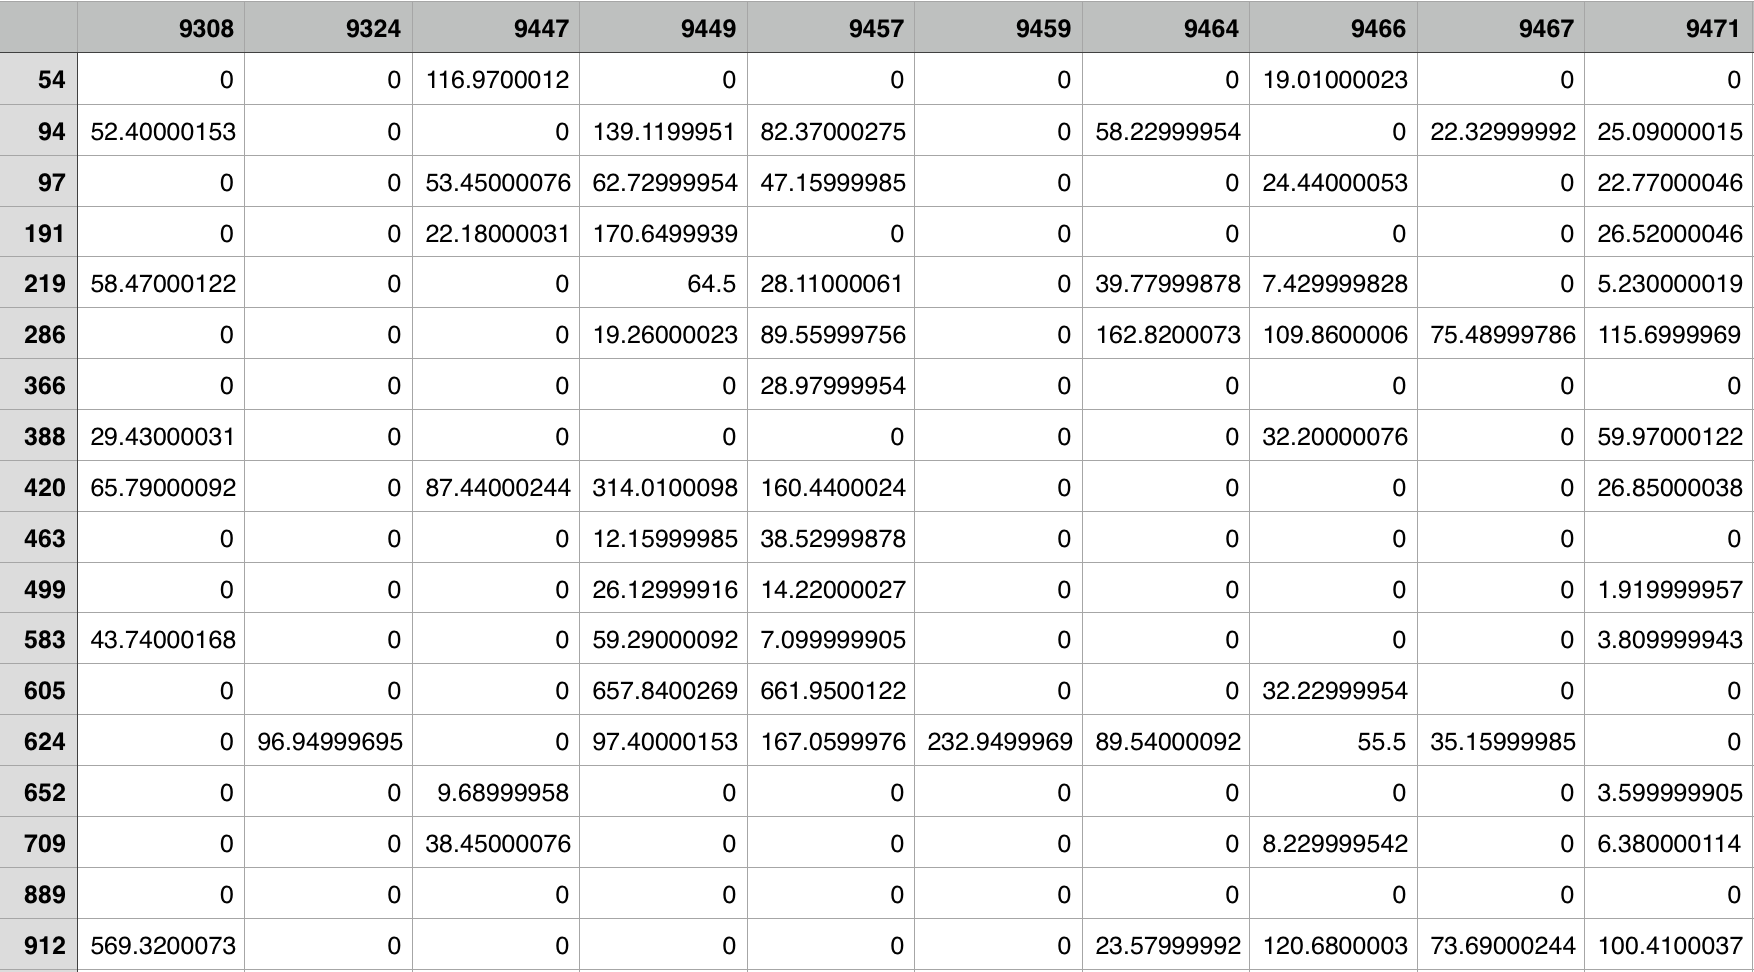
\includegraphics{feature.png}
  \caption{Example of 'feature.csv' pattern}
  \label{example feature}
\end{figure}
\begin{figure}[ht]
  \centering
  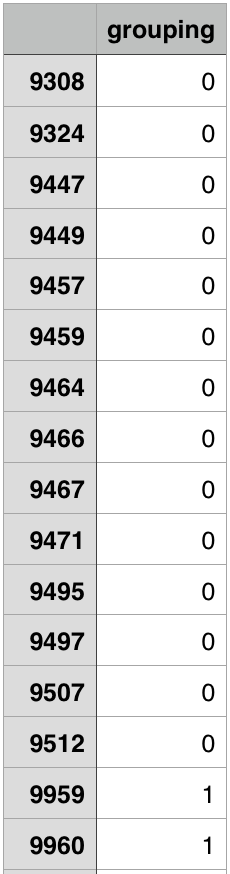
\includegraphics[width=2cm]{group.png}
  \caption{Example of 'group.csv' pattern}
  \label{example group}
\end{figure}


After creating the two csv.files, we need the paths for the two csv.files:

\begin{Schunk}
\begin{Sinput}
> path1 <- "/path/to/your/feature.csv/"
> path2 <- "/path/to/your/group.csv/"
\end{Sinput}
\end{Schunk}

Here for demonstration purposes, we use the data in the {\tt SDAMS} package

\begin{Schunk}
\begin{Sinput}
> directory1 <- system.file("extdata", package="SDAMS", mustWork=TRUE)
> path1<-paste(directory1,"ProstateFeature.csv",sep="/")
> directory2 <- system.file("extdata", package="SDAMS", mustWork=TRUE)
> path2<-paste(directory2,"ProstateGroup.csv",sep="/")
\end{Sinput}
\end{Schunk}

then use the function {\tt getMSsetfromCSV} after loading the {\tt SDAMS}
package
\begin{Schunk}
\begin{Sinput}
> library("SDAMS")
> exampleMSset1 = createMSsetfromCSV(path1,path2)
> exampleMSset1
\end{Sinput}
\begin{Soutput}
MSset (storageMode: lockedEnvironment)
assayData: 560 features, 202 samples 
  element names: exprs 
protocolData: none
phenoData
  sampleNames: 9512 9963 ... 49586 (202 total)
  varLabels: grouping
  varMetadata: labelDescription
featureData: none
experimentData: use 'experimentData(object)'
Annotation:  
\end{Soutput}
\begin{Sinput}
> head(featuredata(exampleMSset1)[,1:10])
\end{Sinput}
\begin{Soutput}
        9512   9963  9965  9975   9979  9997 10015  10034  10044 10047
93922   0.00   0.00  0.00  0.00   0.00  0.00 68.97   0.00   0.00  0.00
87209   0.00   0.00  0.00  0.00   0.00  0.00  0.00   0.00   0.00 43.87
29633   0.00   0.00  0.00  0.00   0.00  0.00  0.00  57.21   0.00  0.00
40225   0.00 226.40  0.00 19.65   0.00  0.00  0.00   0.00   0.00  0.00
126342  0.00   0.00  0.00  0.00   0.00 20.43  0.00   0.00 109.93  0.00
42832  52.32 137.76 70.25  0.00 453.23 92.20  0.00 352.55 496.71  0.00
\end{Soutput}
\begin{Sinput}
> head(phenotypedata(exampleMSset1))
\end{Sinput}
\begin{Soutput}
     grouping
9512        0
9963        1
9965        1
9975        1
9979        1
9997        1
\end{Soutput}
\end{Schunk}



\subsection{Create MSset from R global environment}
If the two datasets have been already claeaned and loaded into the R global
environment, we can use {\tt createMSsetFromEnvir} to create a {\tt MSset} object.

\begin{Schunk}
\begin{Sinput}
> set.seed(100)
> featureInfo = matrix(runif(800,-2,5),ncol = 40)
> featureInfo[featureInfo<0] = 0
> rownames(featureInfo) = paste("feature",1:20,sep = '')
> colnames(featureInfo) = paste('subject',1:40,sep = '')
> groupInfo = data.frame(grouping=matrix(sample(0:1,40,replace = TRUE),ncol = 1))
> rownames(groupInfo)=colnames(featureInfo)
> exampleMSset2 = createMSsetFromEnvir(feature = featureInfo,group = groupInfo)
> exampleMSset2
\end{Sinput}
\begin{Soutput}
MSset (storageMode: lockedEnvironment)
assayData: 20 features, 40 samples 
  element names: exprs 
protocolData: none
phenoData
  sampleNames: subject1 subject2 ... subject40 (40 total)
  varLabels: grouping
  varMetadata: labelDescription
featureData: none
experimentData: use 'experimentData(object)'
Annotation:  
\end{Soutput}
\begin{Sinput}
> head(featuredata(exampleMSset2)[,1:10])
\end{Sinput}
\begin{Soutput}
          subject1  subject2  subject3  subject4 subject5  subject6  subject7
feature1 0.1543628 1.7506781 0.3146237 1.2459082 1.216678 0.2919056 0.7766364
feature2 0.0000000 2.9756269 4.0558438 2.5297084 2.195787 0.7263509 0.7489158
feature3 1.8662570 1.7684409 3.4430911 4.7240116 4.438053 0.0000000 1.3078982
feature4 0.0000000 3.2428056 3.7911241 2.7347872 4.879769 0.5297764 2.0855984
feature5 1.2798450 0.9407102 2.2232705 1.1160362 0.000000 1.9968466 0.4667102
feature6 1.3863951 0.0000000 1.4386228 0.5044165 2.045562 2.7941617 0.0000000
         subject8 subject9  subject10
feature1 2.712745 3.705652 0.02105356
feature2 0.000000 1.978800 3.02481591
feature3 0.000000 1.360440 4.46378210
feature4 4.359349 0.000000 2.72457641
feature5 0.000000 0.000000 0.00000000
feature6 3.102040 0.000000 0.43647014
\end{Soutput}
\begin{Sinput}
> head(phenotypedata(exampleMSset2))
\end{Sinput}
\begin{Soutput}
         grouping
subject1        0
subject2        0
subject3        0
subject4        1
subject5        1
subject6        0
\end{Soutput}
\begin{Sinput}
> 
\end{Sinput}
\end{Schunk}

\section{Data Analysis}

Finally, we perform differential abundance analyais using {\tt MSset} created in
the last section. This can be done by using function {\tt SDA}. And a list with
point estimates, p-values, q-values and corresponding feature names is returned.
Below is results generated by using the {\tt MSset} exampleMSset1.

\begin{Schunk}
\begin{Sinput}
> results = SDA(exampleMSset1)
> head(results$gamma)
\end{Sinput}
\begin{Soutput}
[1]  0.1100009  0.8629447 -0.7151261  0.2876821 -0.1251631  0.6292037
\end{Soutput}
\begin{Sinput}
> head(results$beta)
\end{Sinput}
\begin{Soutput}
[1] -0.04912170 -1.11354659 -1.30566809  0.02484749  0.53967121 -0.22075205
\end{Soutput}
\begin{Sinput}
> head(results$qv_gamma)
\end{Sinput}
\begin{Soutput}
[1] 0.4092097 0.1914385 0.2191259 0.3505466 0.3887992 0.1651784
\end{Soutput}
\begin{Sinput}
> head(results$qv_beta)
\end{Sinput}
\begin{Soutput}
[1] 0.7466379 0.2979437 0.2525717 0.7599717 0.2673415 0.3235222
\end{Soutput}
\begin{Sinput}
> head(results$qv_2part)
\end{Sinput}
\begin{Soutput}
          [,1]
[1,] 0.4622205
[2,] 0.1380966
[3,] 0.1192246
[4,] 0.4323376
[5,] 0.1806273
[6,] 0.1345612
\end{Soutput}
\begin{Sinput}
> head(results$feat.names)
\end{Sinput}
\begin{Soutput}
[1] "93922"  "29633"  "40225"  "126342" "42832"  "127351"
\end{Soutput}
\end{Schunk}



\section{Session Info}

\begin{Schunk}
\begin{Sinput}
> toLatex(sessionInfo())
\end{Sinput}
\begin{itemize}\raggedright
  \item R version 3.4.3 (2017-11-30), \verb|x86_64-apple-darwin15.6.0|
  \item Locale: \verb|en_US.UTF-8/en_US.UTF-8/en_US.UTF-8/C/en_US.UTF-8/en_US.UTF-8|
  \item Running under: \verb|macOS High Sierra 10.13.1|
  \item Matrix products: default
  \item BLAS: \verb|/Library/Frameworks/R.framework/Versions/3.4/Resources/lib/libRblas.0.dylib|
  \item LAPACK: \verb|/Library/Frameworks/R.framework/Versions/3.4/Resources/lib/libRlapack.dylib|
  \item Base packages: base, datasets, graphics, grDevices, methods,
    stats, utils
  \item Other packages: SDAMS~0.99.4
  \item Loaded via a namespace (and not attached): Biobase~2.36.2,
    BiocGenerics~0.22.1, colorspace~1.3-2, compiler~3.4.3,
    ggplot2~2.2.1, grid~3.4.3, gtable~0.2.0, lazyeval~0.2.0,
    magrittr~1.5, munsell~0.4.3, parallel~3.4.3, plyr~1.8.4,
    qvalue~2.8.0, Rcpp~0.12.11, reshape2~1.4.2, rlang~0.1.1,
    scales~0.4.1, splines~3.4.3, stringi~1.1.5, stringr~1.2.0,
    tibble~1.3.3, tools~3.4.3, trust~0.1-7
\end{itemize}\end{Schunk}


\bibliography{reference}


\end{document}
